\chapter{Metodología y fases del producto}
\label{metodologia}
\section{Metodología}
La metodología escogida para llevar a cabo el proyecto es la \textbf{scrum}, a pesar de
estar orientada al trabajo en equipo nos propone una forma de estructurar las tareas y
las difentes iteraciones que nos puede facilitar el trabajo a la hora de desarrollar las
diversas partes del producto. Algunas de las características que tendrán más peso en el
desarrollo son estas:

El uso de \textbf{iteraciones} para dividir la carga de trabajo y agrupar tareas,
el desarrollo de la aplicación se dividirá en una serie de etapas con el objetivo de
orientar cada una de ellas a desarrollar una o varias funcionalidades del producto, con
esto conseguimos acotar la duración de algunas tareas y marcamos objetivos a corto/medio
plazo.
	
División del trabajo en \textbf{tareas cortas}, el hecho de tener objetivos a
corto/medio plazo nos obliga a dividir las tareas en una serie de objetivos lo más
pequeños posibles, esto permite obtener una sensación de éxito de forma rápida lo cual
ayuda a mantener una moral y motivación altas. 

Para acompañar y ayudar a la planificación del trabajo usaremos la herramienta `Trello'
~\ref{img:logo_trello} \footnote{Página de `Trello': https://trello.com/es}
la cual nos permitirá crear distintas listas según el propósito o el estado de
desarrollo de las distintas tareas que contentendrán, cada tarea se ve representada con
una tarjeta la cual puede tener una serie de subtareas asociadas dentro. Esto nos
permitirá tener un registro de todas las labores que quedan por hacer en la iteración y
cuales ya estan termiandas completamente o sólo parcialmente, además de poder conservar
las listas de las tareas realizadas en iteraciones anteriores para futuras revisiones.

\begin{figure}[ht]
\centering

\includegraphics[width=0.45\textwidth]{imagenes/metodologia/logo-trello.png}
\caption{Logo de `Trello'.}
\label{img:logo_trello}
\end{figure}

Otra herramienta de control que usaremos durante el desarrollo será `Toggl'
~\ref{img:logo_toggl} \footnote{Página de `Toggl': https://toggl.com}
la cual nos permitirá llevar a cabo un registro de las horas que dedicamos en cada tarea
y agrupar tareas en función del campo de estudio o parte del desarrollor al que pertecen.

\begin{figure}[ht]
\centering

\includegraphics[width=0.45\textwidth]{imagenes/metodologia/logo-toggl.png}
\caption{Logo de `Toggl'.}
\label{img:logo_toggl}
\end{figure}

\section{Iteraciones}
En esta sección vamos proceder a comentar brevemente la intención y las tareas que se
han llevado a cabo en cada iteración adjuntando también el panel de `Trello' asociado.

\subsection{Iteración 0}
Esta iteración tenía como proposito terminar de definir la idea que teniamos para el
proyecto, ya que, todavía era un poco difuso el producto final que se quería desarrollar.
Para ir entrando en una dinámica productiva e ir definiendo lo que se quería hacer,
comenzamos por iniciar el desarrollo de un propotipo a la vez que preparabamos un poco
los materiales relacionados con la memoria, como puede ser la lectura de las directrices
y/o la revisión de la plantilla de \LaTeX~\ref{img:it_0}.

\begin{figure}[ht]
\centering
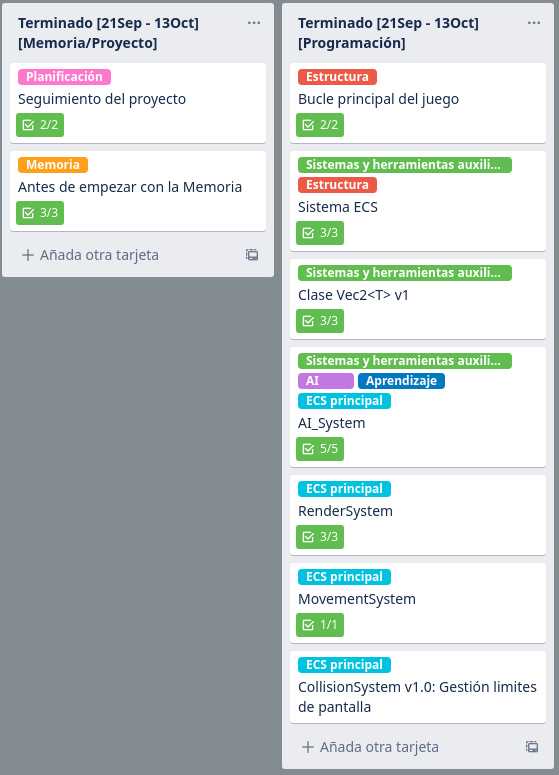
\includegraphics[width=0.45\textwidth]{imagenes/metodologia/tareas_it0.png}
\caption{Lista de tareas realizadas en la iteración 0}
\label{img:it_0}
\end{figure}

\subsection{Iteración 1}
A lo largo de esta iteración se siguió añadiendo sistemas al prototipo y se comenzó a
trabajar en la \ac{IA} del juego creando los primeros comportamientos y herramientas
para cambiar entre ellos, además finalizamos la introducción en el uso de \LaTeX y la
plantilla comenzando así con la redacción de esta memoria~\ref{img:it_1}.

\begin{figure}[ht]
\centering
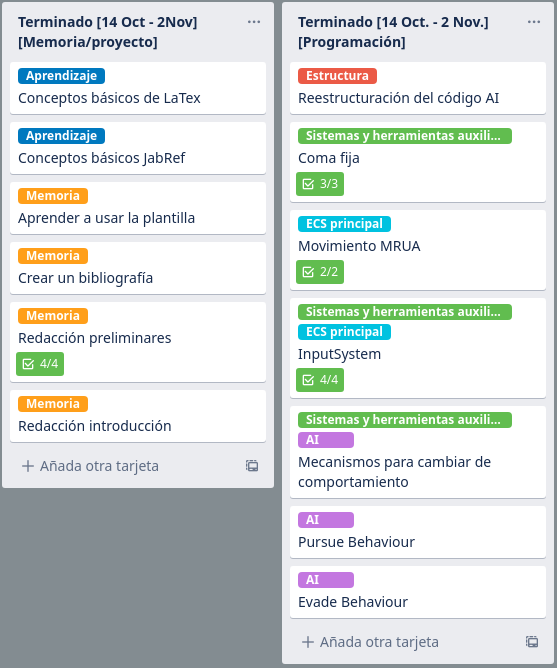
\includegraphics[width=0.45\textwidth]{imagenes/metodologia/tareas_it1.png}
\caption{Lista de tareas realizadas en la iteración 1}
\label{img:it_1}
\end{figure}


